\documentclass[aspectratio=169]{beamer}
\newif\ifdraft
\draftfalse
\usepackage{style}
\addbibresource{references.bib}
\title[Title]{Erdős--Szekeres theorem for multidimensional arrays}
\subtitle{ Matija Bucić · Benny Sudakov · Tuan Tran}

% \subtitle{Subtitle}

\author{Andrzej Antoni Kwaśniewski \\ 
Advisor: Krystian Gajdzica}
\date[]{Combinatorics 8 V 2026}
\begin{document}
\onehalfspacing
%---------------------------------------------------------
\mysimplefootline

\frame{\titlepage}

%---------------------------------------------------------
\section{Preliminaries}
\begin{frame}{}
    \begin{theorem}{ Erd\H{o}s--Szekeres theorem (1935)}
        Any sequence of \((n-1)(m-1)+1\) distinct real numbers contains either an increasing sequence of length \(n\) or a decreasing subsequence of length \(m\).
    \end{theorem}
    \pause
    \begin{proof}{Proof}
        \begin{columns}
        \begin{column}{0.75\linewidth}
        Label each number \(n_i\) in the sequence with the pair \((a_i,b_i)\)
        \begin{itemize}
            \item \(a_i\) - length of the longest increasing subsequence ending at \(n_i\)
            \item \(b_i\) - length of the longest decreasing subsequence ending at \(n_i\)
        \end{itemize}
        \pause
        Each \(n_i\) has a distinct pair \((a_i,b_i)\)\\
        \begin{itemize}
            \item if \(i<j\) and \(n_i<n_j\) then \(a_i<a_j\)
            \item if \(i<j\) and \(n_i>n_j\) then \(b_i<b_j\)
        \end{itemize}
        \end{column}
        \begin{column}{0.2\linewidth}
            \begin{figure}
                \centering
                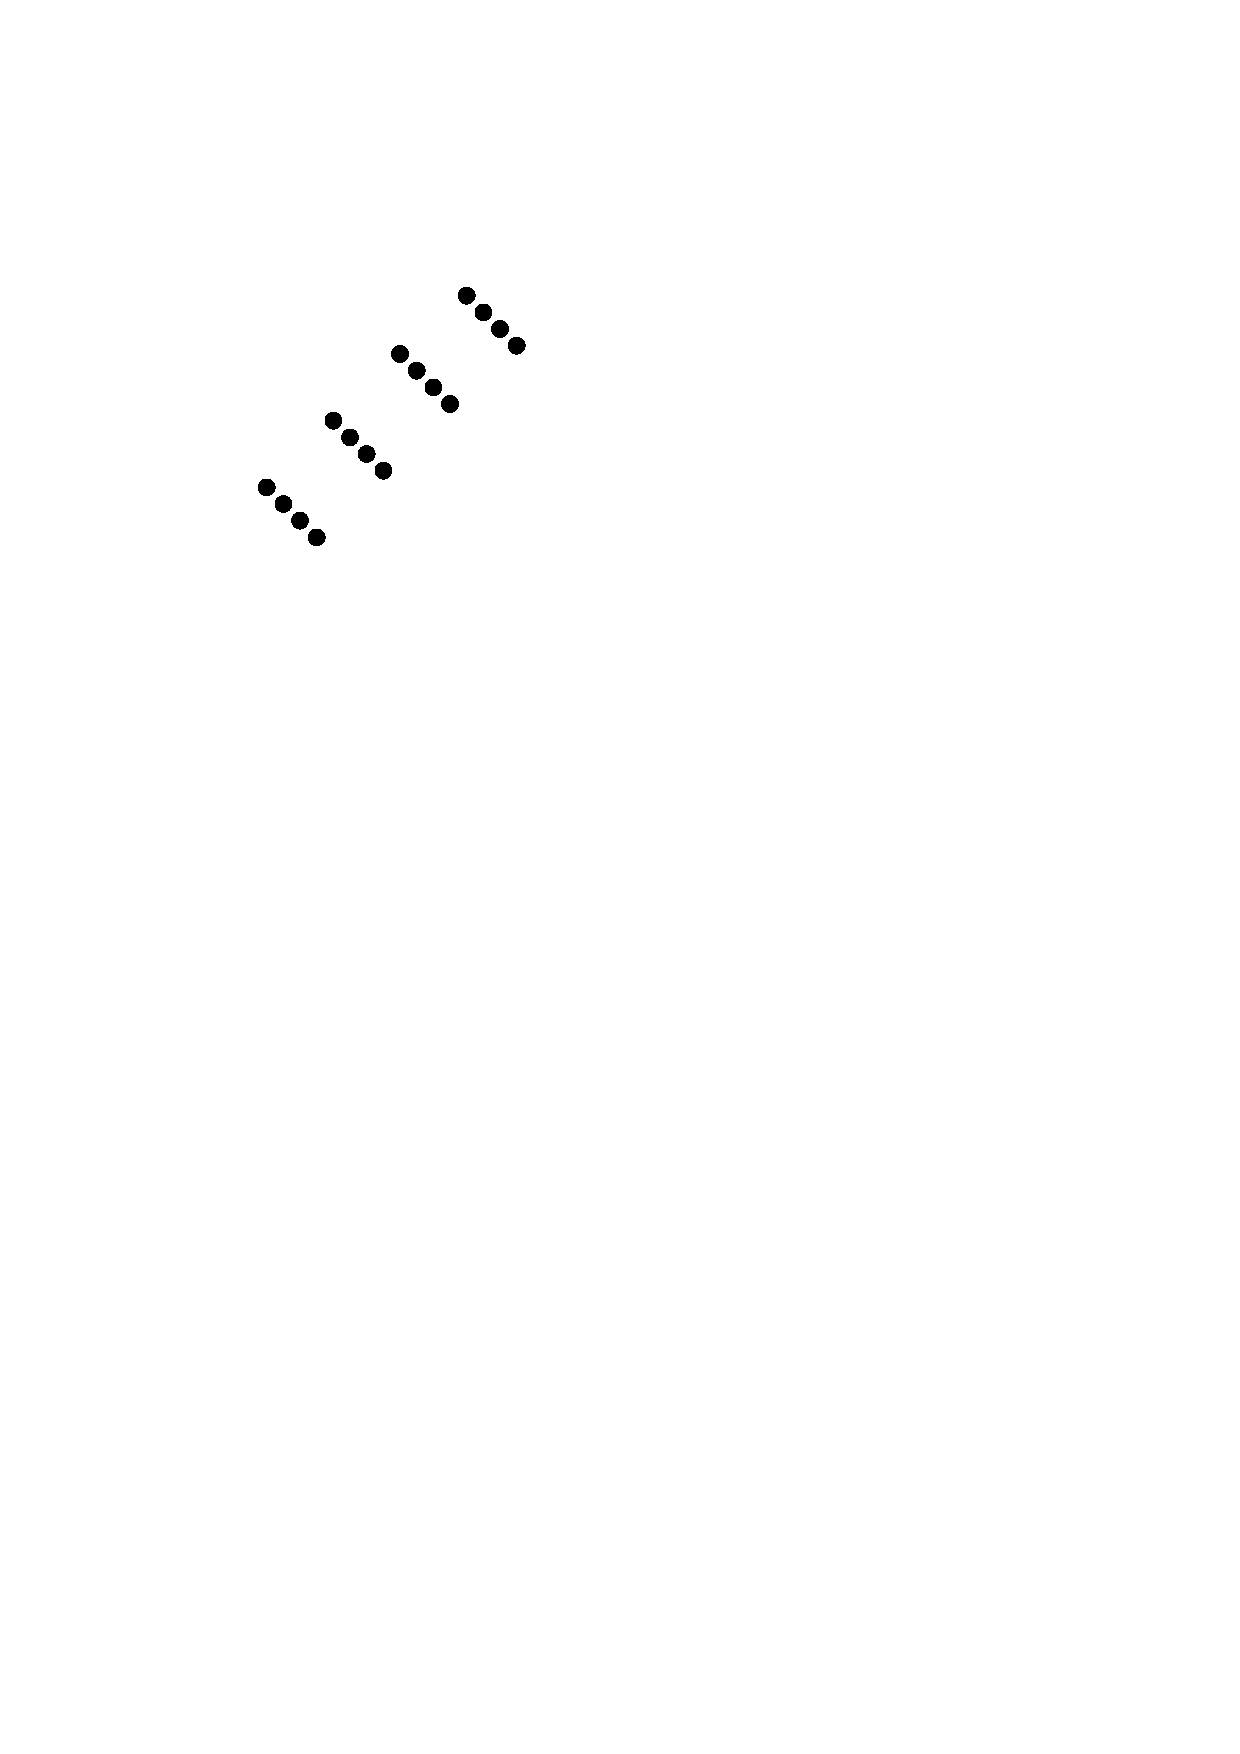
\includegraphics[width=0.8\linewidth]{images/esz.pdf}
            \end{figure}
        \end{column}
        \end{columns}
        \pause
        If \(a_i<n,b_i<m\) then there are at most \((n-1)(m-1)\) values, but there are \((n-1)(m-1)+1\) numbers thus contradiction.
    \end{proof}
\end{frame}

\begin{frame}
    % \begin{theorem}{Dilworth's Lemma}
    %     In any finite partially ordered set, the maximum size of an antichain equals the minimum number of chains needed to partition the set.
    % \end{theorem}
    \begin{theorem}{High-Order Monotonicity}
        A $(k+1)$-tuple is positive if its $k$-th derivative is nonnegative. A set is $k$-th order monotone if all its $(k+1)$-tuples are positive or all negative.
    \end{theorem}
    \begin{theorem}{Suk, 2017}
        Any $2^{n+o(n)}$ points in $\mathbb{R}^2$ contain a convex subset of size $n$.
    \end{theorem}
    \begin{theorem}{Xu, 2024}
        Any sequence of $n$ pairwise distinct real numbers contains a $k$-modal subsequence of length at least $\sqrt{(2k + 1)(n - \frac{1}{4})} - \frac{k}{2}$.
    \end{theorem}

\end{frame}

\begin{frame}{}
  \begin{ffact}{Array}
    A \textit{d-dimensional array} is an injective function
    \[
      f : A_1 \times \cdots \times A_d \to \mathbb{R},
    \]
    where \( A_1, \ldots, A_d \subseteq \mathbb{Z} \) are non-empty finite sets.
    We say \( f \) has size \( |A_1| \times \cdots \times |A_d| \).
  \end{ffact}
    \pause
  \medskip
  \begin{ffact}{Monotone Array}
    A \( d \)-dimensional array \( f \) is \textbf{monotone} if for each
    coordinate direction \( i \in [d] \), \emph{all} one-dimensional slices
    in direction \( i \) are increasing, \emph{or} all are decreasing.
  \end{ffact}
\end{frame}

\begin{frame}{Inconsistently Monotone Arrays}
  \begin{ffact}{Inconsistently monotone array}
    A \( d \)-dimensional array is \textbf{inconsistently monotone} if every
    one-dimensional slice is monotone (but slices along the same direction
    may go in different directions).
  \end{ffact}
\end{frame}


\begin{frame}{}
  \begin{ffact}{Lex--Monotone Array}
    A \( d \)-dimensional array \( f \) is \textbf{lex--monotone} if there exist
    a permutation \( \sigma : [d] \to [d] \) and signs \( s \in \{-1,+1\}^d \) such that
    \[
      f(x) < f(y) \;\iff\;
      \bigl(s_{\sigma(1)}\,x_{\sigma(1)},\ldots,s_{\sigma(d)}\,x_{\sigma(d)}\bigr)
      <_{\mathrm{lex}}
      \bigl(s_{\sigma(1)}\,y_{\sigma(1)},\ldots,s_{\sigma(d)}\,y_{\sigma(d)}\bigr).
    \]
  \end{ffact}
\end{frame}
\begin{frame}{Applications of lex--monotone arrays}
        \begin{hheading}{Poset dimension theory} lex--monotone arrays arise as realizers 
            of partial orders of bounded dimension
            \begin{itemize}
                \item Felsner, Fishburn, Trotter -- \textit{Finite three-dimensional partial 
                orders which are not sphere orders} (1999)
            \end{itemize}
        \end{hheading}
        \begin{hheading}{Temporal constraint satisfaction problem} lex--monotone structure 
            is used to determine the complexity of deciding temporal CSPs
            \begin{itemize}
                \item Bodirsky, K\'{a}ra -- \textit{The complexity of temporal constraint 
                satisfaction problems} (2010)
            \end{itemize}
        \end{hheading}
\end{frame}
\begin{frame}{}
    Our proofs work like:
    \vspace{-0.5cm}
\[
\text{Array} 
\rightarrow
\text{Inc. monotone}
\rightarrow
\text{Monotone}
\rightarrow
\text{Lex--monotone}
\]
\end{frame}
\section{Monotone arrays}



% ----------------------------


% \begin{frame}{Lower bounds on  \( M_d(n) \)}
%   \begin{itemize}
%     \item \( M_1(n) = (n-1)^2 + 1 \) (E.SZ).
%     \item  \( M_d(n) \geq n^{(1-1/d)\,n^{d-1}} \)
%   \end{itemize}
%   \pause
%   \begin{proof}{Probabilistic proof}
%       Take \(d=2\), then the bound becomes \(M_2(n)\geq n^{n/2}\).\\
%       Expected number of monotone subarrays of size \(n\) is:
%       \[E=\binom{N}{n}\binom{N}{n}\left(\frac{1}{n!}\right)^n \ll 1\]
%   \end{proof}
% \end{frame}


% ----------------------------


\begin{frame}{}
    \( M_d(n) \): minimum \( N \) such that every \( d \)-dim
  \( N^d \) array has a monotone \( n^d \) subarray.
  \begin{itemize}
    \item $M_1(n) = (n-1)^2 + 1$ \quad (Erd\H{o}s--Szekeres)
    \item $M_d(n) \geq n^{(1-1/d)\,n^{d-1}}$
  \end{itemize}
  \pause
  \begin{proof}{Probabilistic proof sketch ($d=2$)}
      The bound becomes $M_2(n) \geq n^{n/2}$. \\
      Take a uniformly random $N \times N$ array. \\
      By linearity of expectations the expected number of monotone 
      $n \times n$ subarrays is at most
      \[
          E \leq \binom{N}{n}^2 \cdot \frac{4}{(n!)^n} 
          \leq \frac{4N^{2n}}{(n!)^n}\ll1.
      \]
      \pause
      Thus there exists an array with no monotone $n\times n$ subarray.
      Thus $M_2(n) \geq n^{n/2}$.
  \end{proof}
\end{frame}

% ----------------------------

\begin{frame}{Upper bounds}
    \begin{fact}{Previous bounds}
    \begin{itemize}
        \item \(M_2(n)\leq \text{towr}_5(n)\)
        \item \(M_d(n)\leq \text{Ackerman}(n)\)
    \end{itemize}
    \pause
    \end{fact}
    \begin{fact}{Authors}
        \item[\textbf{(i)}] \( \displaystyle M_2(n) \leq 2^{2^{(2+o(1))n}} \)
      \item[\textbf{(ii)}] \( \displaystyle M_3(n) \leq 2^{2^{(2+o(1))n^2}} \)
      \item[\textbf{(iii)}] \( \displaystyle M_d(n) \leq 2^{2^{2^{O_d(n^{d-1})}}}
            \quad \text{for } d \geq 4 \)
    \end{fact}
\end{frame}

% ----------------------------

\begin{frame}{Proof of the bound for \(M_2(n) \le 2^{2^{2n}}\)}
\begin{columns}
\begin{column}{0.65\linewidth}

Take \(N = 2^{2^{2n}}\) and an array of size \(4n^2 \times N\).

By Erdős--Szekeres, each column contains a monotone subsequence of length \(2n\).\\
\onslide<2->{
There are at most \(\binom{4n^2}{2n}\) possible choices of positions, so by pigeonhole,
there exists a set \(R\) of \(2n\) rows and a set \(C\) of columns with
\[
|C| \ge \frac{N}{\binom{4n^2}{2n}} \approx N^{1-o(1)}
\]
such that all columns in \(C\) are monotone on \(R\).\\
}
\onslide<3->{
At least half of these are increasing (or decreasing), so we may assume all columns
in \(C\) are increasing.
}
\end{column}

\begin{column}{0.4\linewidth}
\begin{figure}
\centering
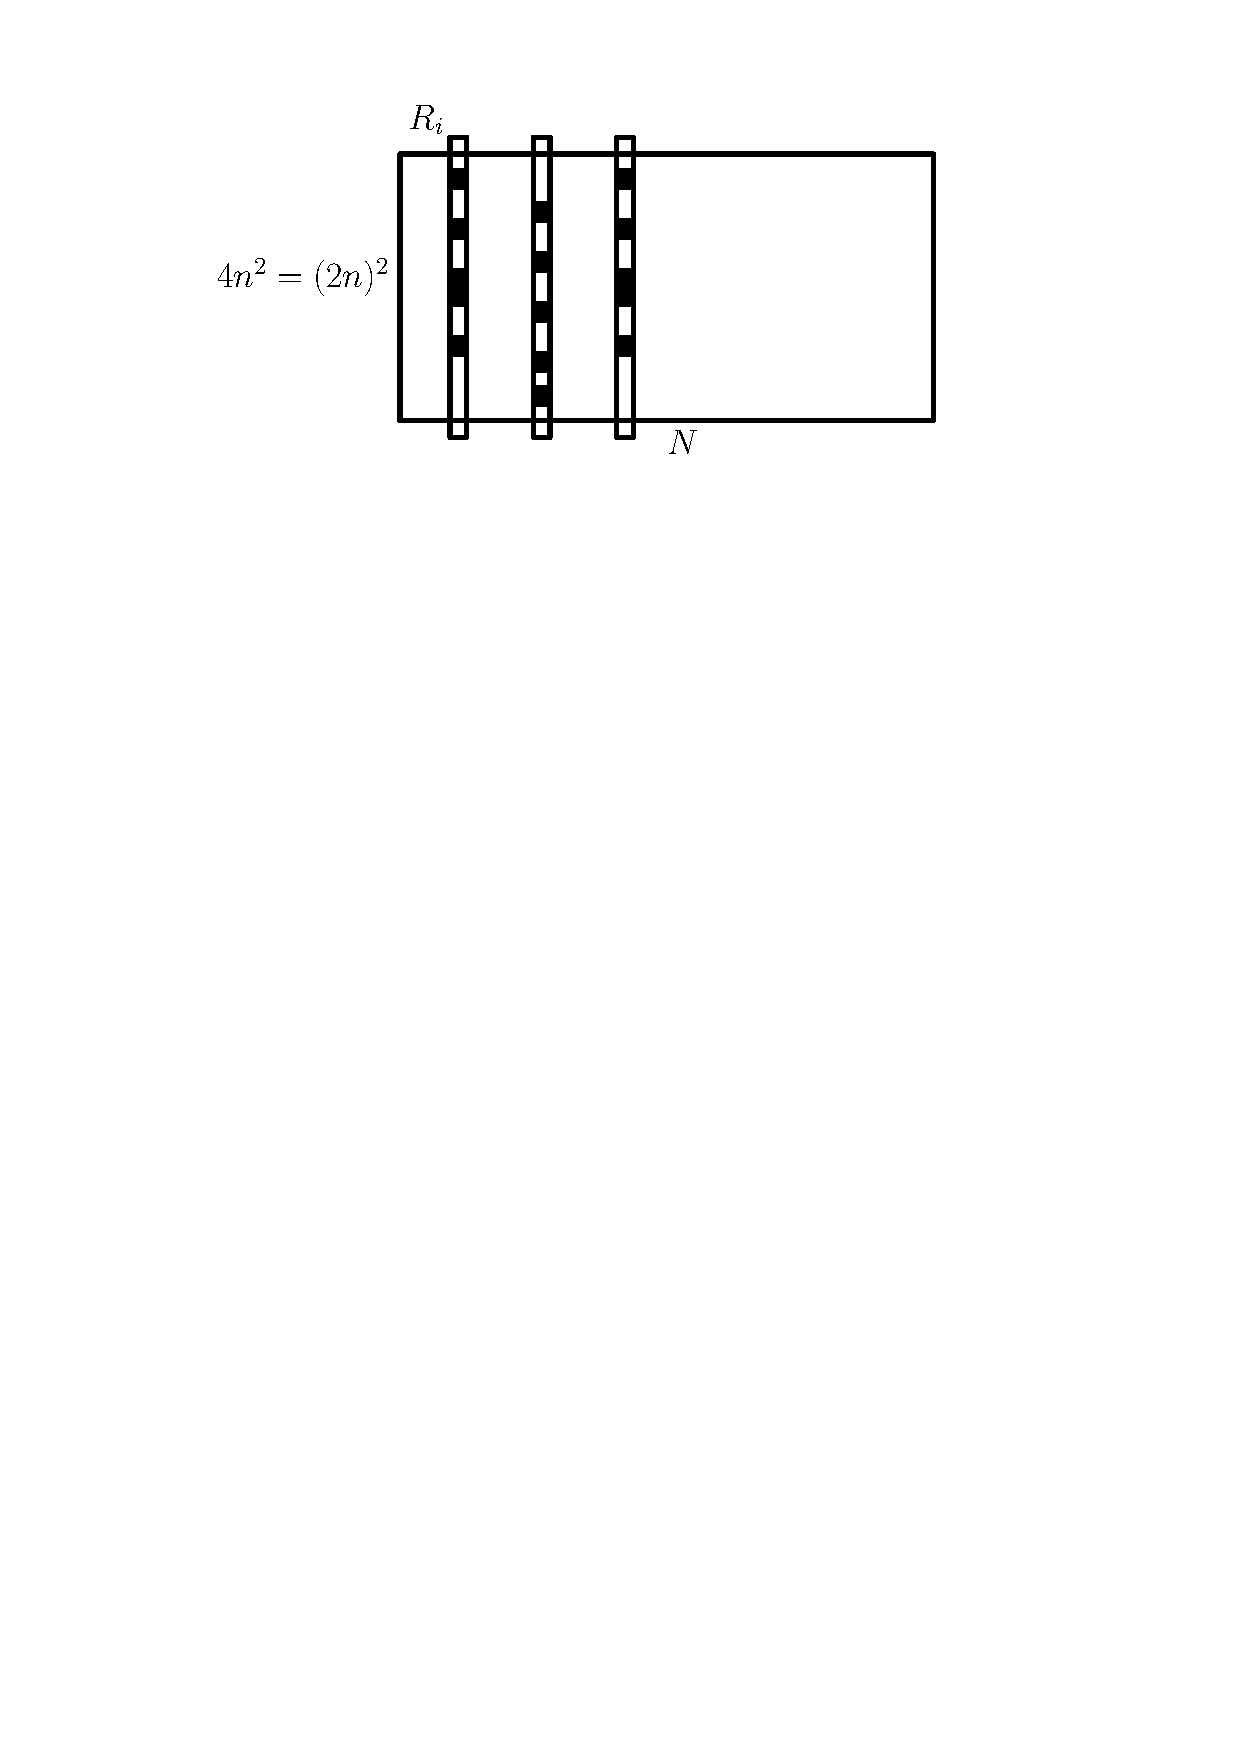
\includegraphics[width=\linewidth]{images/m2_1.pdf}
\end{figure}
\end{column}
\end{columns}
\end{frame}
% ----------------------------


\begin{frame}{Proof of the bound for \(M_2(n) \le 2^{2^{2n}}\)}
\begin{columns}
\begin{column}{0.65\linewidth}
Now iterate Erdős--Szekeres on rows:

At step \(i\), restrict to columns \(C_i\) such that the first \(i\) rows are monotone.
Then
\[
|C_i| \ge |C|^{1/2^i}.
\]
\onslide<2->{
After \(2n\) steps,
\[
|C_{2n}| \ge |C|^{1/2^{2n}} \approx N^{1/2^{2n}}\ge 2n.
\]
}
\onslide<3->{
Thus we obtain a \(2n \times 2n\) subarray where all rows and columns are monotone.
Taking a majority direction among rows gives an \(n \times n\) monotone subarray.
}
\end{column}

\begin{column}{0.4\linewidth}
\begin{figure}
\centering
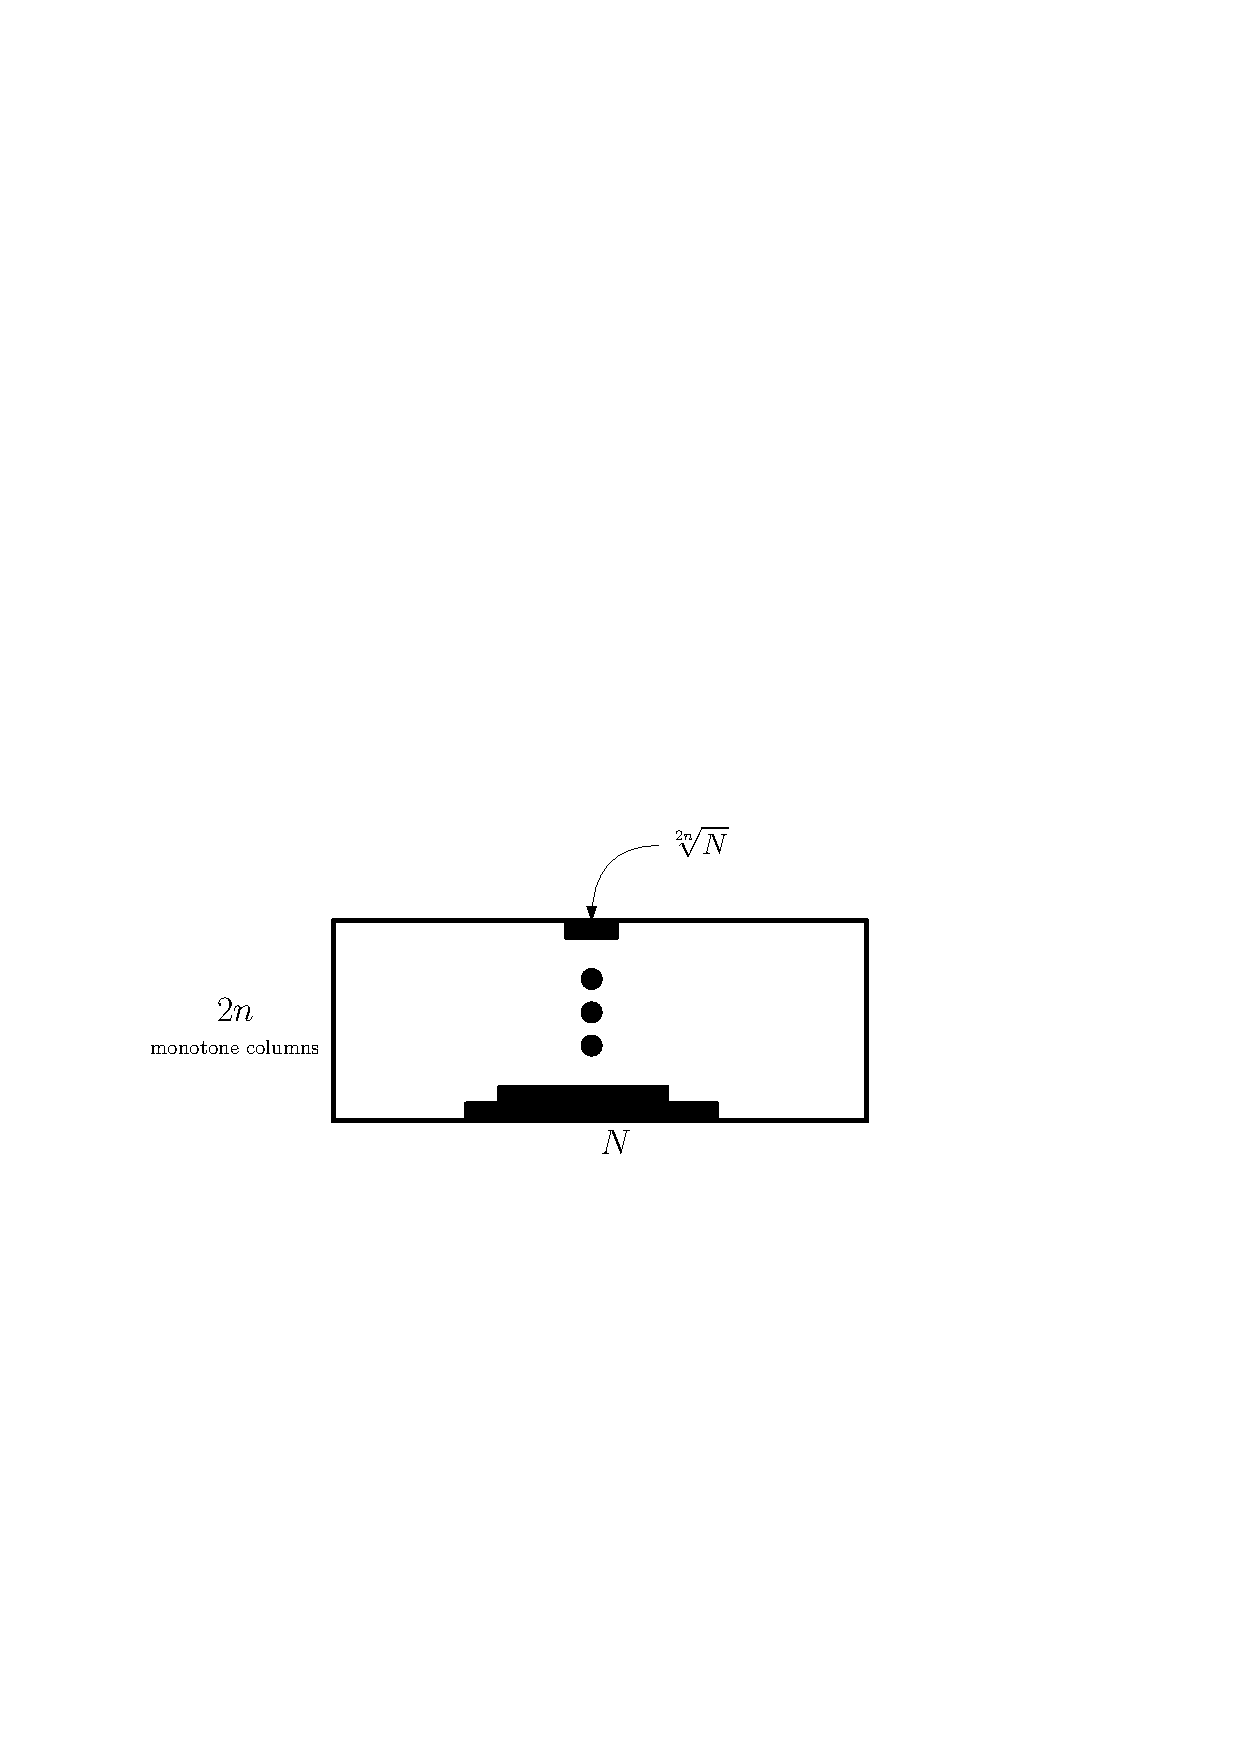
\includegraphics[width=\linewidth]{images/m2_2.pdf}
\end{figure}
\end{column}

\end{columns}
\end{frame}


% ----------------------------


\begin{frame}{Inconsistently Monotone Arrays}
  \begin{ffact}{Inconsistently Monotone Arrays}
    A \( d \)-dimensional array is \textbf{inconsistently monotone} if every
    one-dimensional slice is monotone (but slices along the same direction
    may go in different directions).
  \end{ffact}

  \medskip
    \( M_d'(n) \): minimum \( N \) such that every \( d \)-dim
  \( N^d \) array has an inconsistently monotone \( n^d \) subarray.
    \medskip
    \[M_2(n)\leq M_2'(2n)\]
    \[M_d'(n)\leq 2^{2^{n^{d-1}}}\]
\end{frame}


% ----------------------------

\begin{frame}{Proof of \(M_d'(n)\leq 2^{2^{n^{d-1}}}\)}
    \[
  M_d'(n) \;\leq\; \binom{M_{d-1}'(n)}{n}^{\!d-1} \cdot n^{2n^{d-1}}
\]
Set \( N = \binom{M_{d-1}'(n)}{n}^{d-1} n^{2n^{d-1}} \) and consider an array \( A : [m]^{d-1} \times [N] =S\times N\). We aim to show an inconsistently monotone array of size \(n\).\\
    \pause
  \begin{ffact}{Step 1 — Pigeonhole over heights}\\
  There are \(\binom{m}{n}^{d-1}\) ways to choose the set \(S\).\\
  Thus by pigeonhole principle, there exists a fixed \( S \) and \( H \subseteq [N] \) with
  \[
    |H| \;\geq\; \frac{N}{\binom{m}{n}^{d-1}} \;=\; n^{2n^{d-1}}.
  \]
  such that \(S\times h\) is inconsistently monotone for all \(h \subseteq H\).
  
  \end{ffact}
\end{frame}
\begin{frame}{}
    \[
  M_d'(n) \;\leq\; \binom{M_{d-1}'(n)}{n}^{\!d-1} \cdot n^{2n^{d-1}}
\]
Set \( N = \binom{M_{d-1}'(n)}{n}^{d-1} n^{2n^{d-1}} \) and consider an array \( A : [m]^{d-1} \times [N] =S\times N\). We aim to show an inconsistently monotone array of size \(n\).\\
  \begin{ffact}{Step 2 — Erd\H{o}s--Szekeres along \( H \).}\\
  Label elements of \( S \) as \( s_1,\ldots,s_{n^{d-1}} \).
  Build a nested chain
  \( H_0 \supseteq H_1 \supseteq \cdots \supseteq H_{n^{d-1}} \)
  with \( |H_i| \geq \sqrt{|H_{i-1}|} \), so that \( \{s_j\}\times H_i \)
  is monotone for \( j = 1,\ldots,i \). After \( n^{d-1} \) steps:
  \vspace{-0.5cm}
  \[
    |H_{n^{d-1}}| \;\geq\; |H|^{1/2^{n^{d-1}}} \;\geq\; n.
  \]
  \vspace{-0.5cm}
  Then \(S \times H_{n^{d-1}} \) is inconsistently monotone.
  \end{ffact}
\end{frame}
\begin{frame}{Proof of \(M_d'(n)\leq 2^{2^{n-1}}\)}
    we proved     \[
  M_d'(n) \;\leq\; \binom{M_{d-1}'(n)}{n}^{\!d-1} \cdot n^{2n^{d-1}}
\]
Then by induction using \(\binom{m}{n}\leq m^n\):
\[M_1'(n)=(n-1)^2+1\]
    \[
      M_d'(n)
      \leq \left(2^{2^{n^{d-2}}}\right)^{(d-1)n}\cdot n^{2n^{d-1}}
      = 2^{(d-1)n\cdot 2^{n^{d-2}}+2n^{d-1}\log_2 n}
      = 2^{2^{n^{d-1}}},
    \]
\end{frame}
% ----------------------------


\begin{frame}{}
    \begin{lemma}{Ramsey theory lemma}
    Given k-colouring of vertices of d-dimensional \(N^d\) array there is an \(n^d\) monochromatic subarray if \(2^{Cn^{d-1}}\), where \(C\) is sufficiently large.
    \end{lemma}
    \pause
    \begin{proof}{Proof sketch d=2}
        \begin{itemize}
            \item Each column is a sequence of $N$ cells coloured with $k$ colours
            \item At step $i$, restrict to columns $C_i$ where the first $i$ rows 
            share the same colour. By pigeonhole $|C_i| \geq |C_{i-1}|/k$
            \pause
            \item After $n$ steps: $|C_n| \geq N/k^n$
            \item Apply pigeonhole again on rows: among $N$ rows, 
            some colour class has $\geq N/k$ rows -- pick $n$ of them
            \item Setting $N \geq n \cdot k^{n+1}$ guarantees an $n \times n$ 
            monochromatic subarray
            \pause
            \item For general $d$: iterate over all $d$ dimensions, 
            losing $k^{n^{d-1}}$ at each step, giving $N \geq 2^{Cn^{d-1}}$
        \end{itemize}
    \end{proof}
\end{frame}


%--------------------


\begin{frame}{}
    \begin{theorem}{From inconsistently to consistently}
        Every inconsistently monotone array \(N^d\) has a motone subarray \(n^d\) if \(N=2^{O(n^{d-1})}\)
    \end{theorem}
    \pause
    \begin{proof}{Proof}
    Take an inconsistently monotone array \(A\).\\
    Colour each point \( a \in A \) with its
      \emph{monotonicity pattern}
      \[
        \mathrm{color}(a) = (s_1,\ldots,s_d) \in \{-1,+1\}^d,
        \quad s_i = \begin{cases} +1 & \text{if direction } i \text{ is increasing at } a \\ -1 & \text{otherwise} \end{cases}.
      \]
      By the Ramsey lemma there exists a monochromatic subarray, it is also a monotone subarray.
    \end{proof}
\end{frame}

%--------------------

\begin{frame}{Getting the bound for \(M_d\)}
    \begin{theorem}{Bound on \(M_d'\)}
        \[M_d'(n)\leq 2^{2^{n-1}}\]
    \end{theorem}
    \begin{theorem}{From inconsistently to consistently}
        Every inconsistently monotone array \(N^d\) has a motone subarray \(n^d\) if \(N=2^{O(n^{d-1})}\)
    \end{theorem}
    \pause
    We can combine those proofs to get that:
    \begin{theorem}{Bound on \(M_d\)}
        \[M_d(n)\leq 2^{2^{2^{O(n^{d-1})}}}\]
    \end{theorem}
\end{frame}
\section{Lext-monotone arrays}
\begin{frame}{}
  \begin{ffact}{Lex--Monotone Array}
    A \( d \)-dimensional array \( f \) is \textbf{lex--monotone} if there exist
    a permutation \( \sigma : [d] \to [d] \) and signs \( s \in \{-1,+1\}^d \) such that
    \[
      f(x) < f(y) \;\iff\;
      \bigl(s_{\sigma(1)}\,x_{\sigma(1)},\ldots,s_{\sigma(d)}\,x_{\sigma(d)}\bigr)
      <_{\mathrm{lex}}
      \bigl(s_{\sigma(1)}\,y_{\sigma(1)},\ldots,s_{\sigma(d)}\,y_{\sigma(d)}\bigr).
    \]
  \end{ffact}
    \pause
  \smallskip
  Every lex--monotone array is monotone, but not vice versa.
  \smallskip
\end{frame}
\begin{frame}{Types of 2 dimensional lex--monotone arrays}
    \begin{figure}
        \centering
        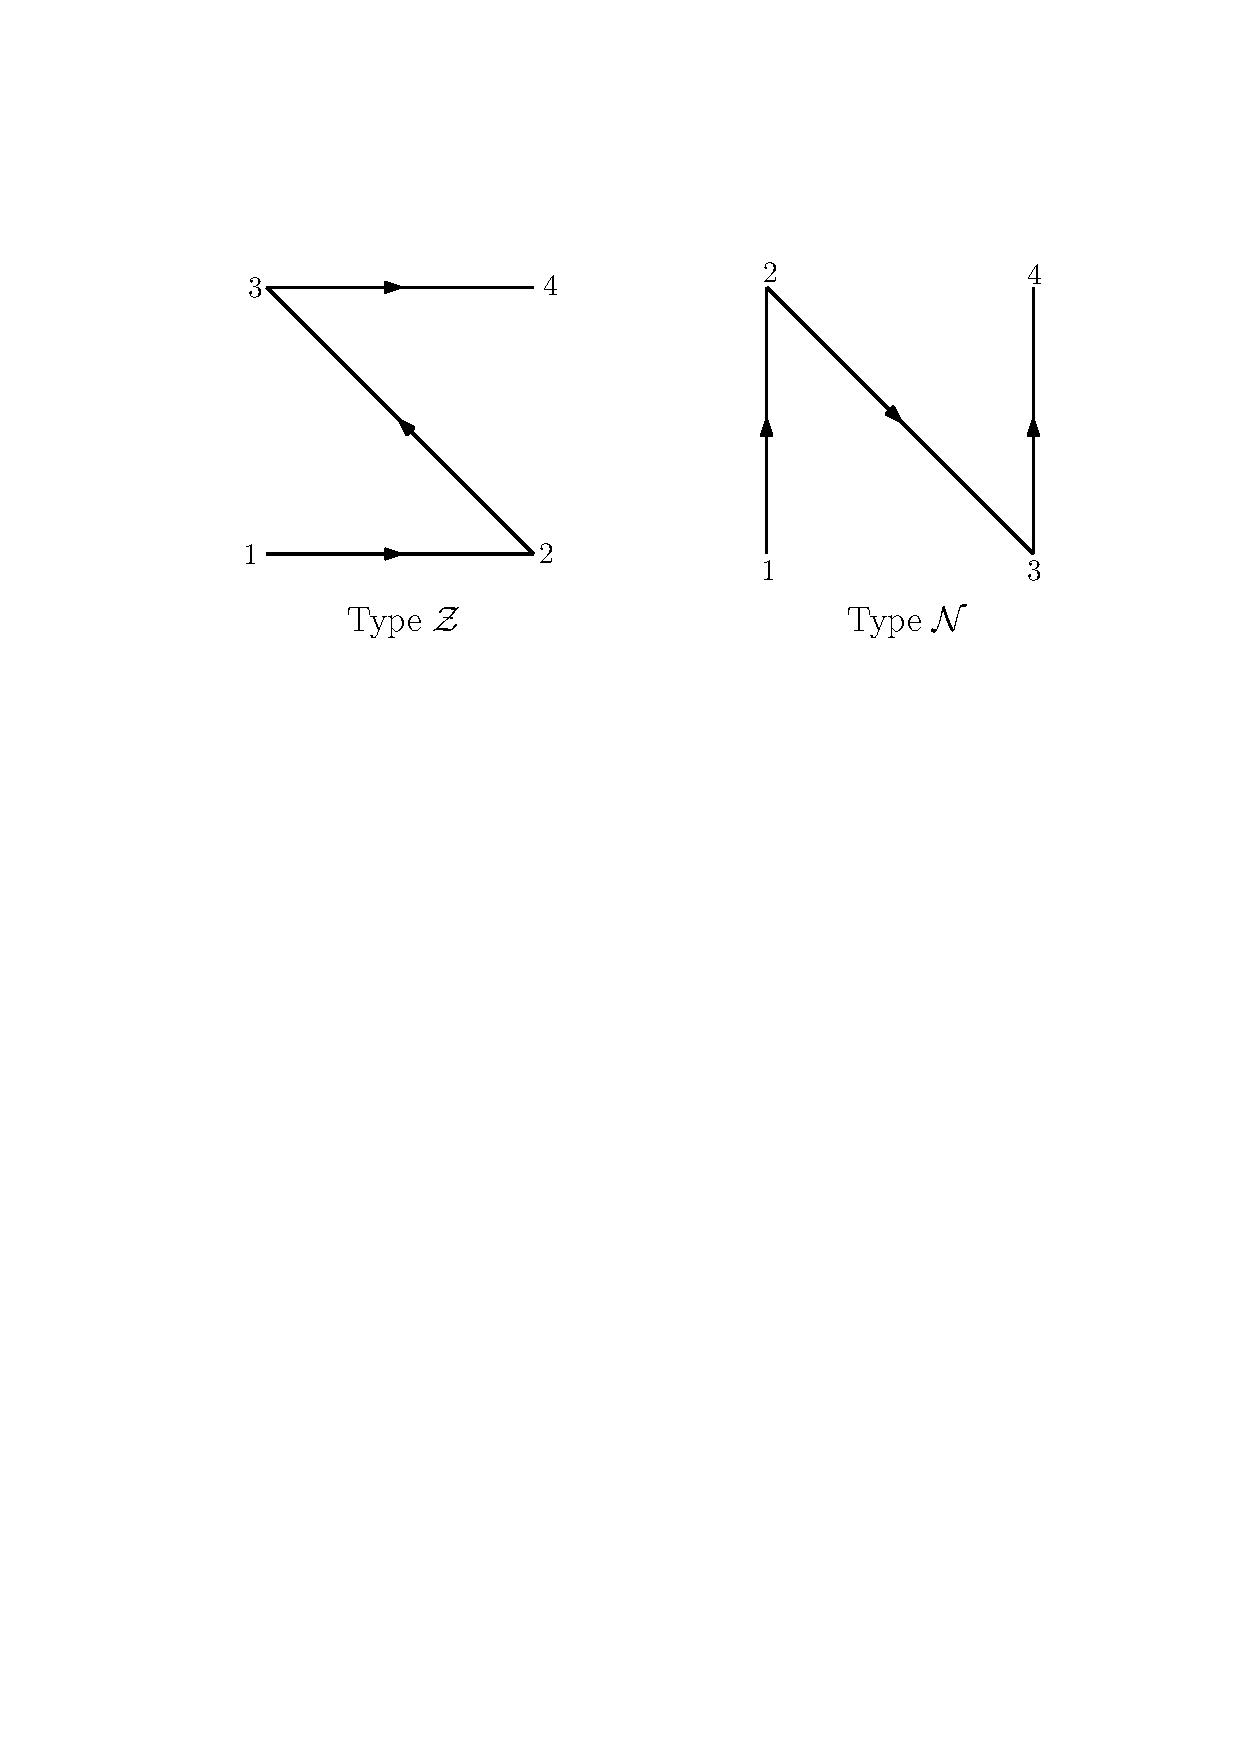
\includegraphics[width=0.9\linewidth]{images/types.pdf}
    \end{figure}
    
\end{frame}
\begin{frame}{Functions \( F_d(n) \) and \( L_d(n) \)}
    \( L_d(n) \): minimum \( N \) such that every \( d \)-dim 
  \( N^d \) array has a lex-monotone \( n^d \) array. \\
  \pause
  \( F_d(n) \): minimum \( N \) such that every \( d \)-dim 
  \( N^d \) monotone array has a lex-monotone \( n^d \) array.
  \pause
  \smallskip
    Obviously \( L_d(n) \leq M_d(F_d(n)) \)\\
    \medskip
    Our proofs work like:
    \vspace{-0.5cm}
\[
\text{Array} 
\xrightarrow{N \geq 2^{2^{n-1}}} 
\text{Inc. monotone}
\xrightarrow{N \geq 2^{O(n^{d-1})}} 
\text{Monotone}
\xrightarrow{F_d(n)} 
\text{Lex--monotone}
\]
\end{frame}
\begin{frame}{\(F_2(n)\leq 2n^2-5n+4\)}
    \begin{columns}
    \begin{column}{0.7\linewidth}
    Let \(f\) be a monotone array \(N^2\), where \(N=(n-1)(2n-3)+1\)\\
    We colour element \((a_i, a_j)\), where \(\set{i,j} \in [1,2n-3]\):
    \begin{itemize}
        \item red if \(f(a_{i+1},a_j)<f(a_i,a_{j+1})\) 
        \item blue if \(f(a_{i+1},a_j)\geq f(a_i,a_{j+1})\) 
    \end{itemize}
    \end{column}
    \begin{column}{0.3\linewidth}
        \begin{figure}
            \centering
            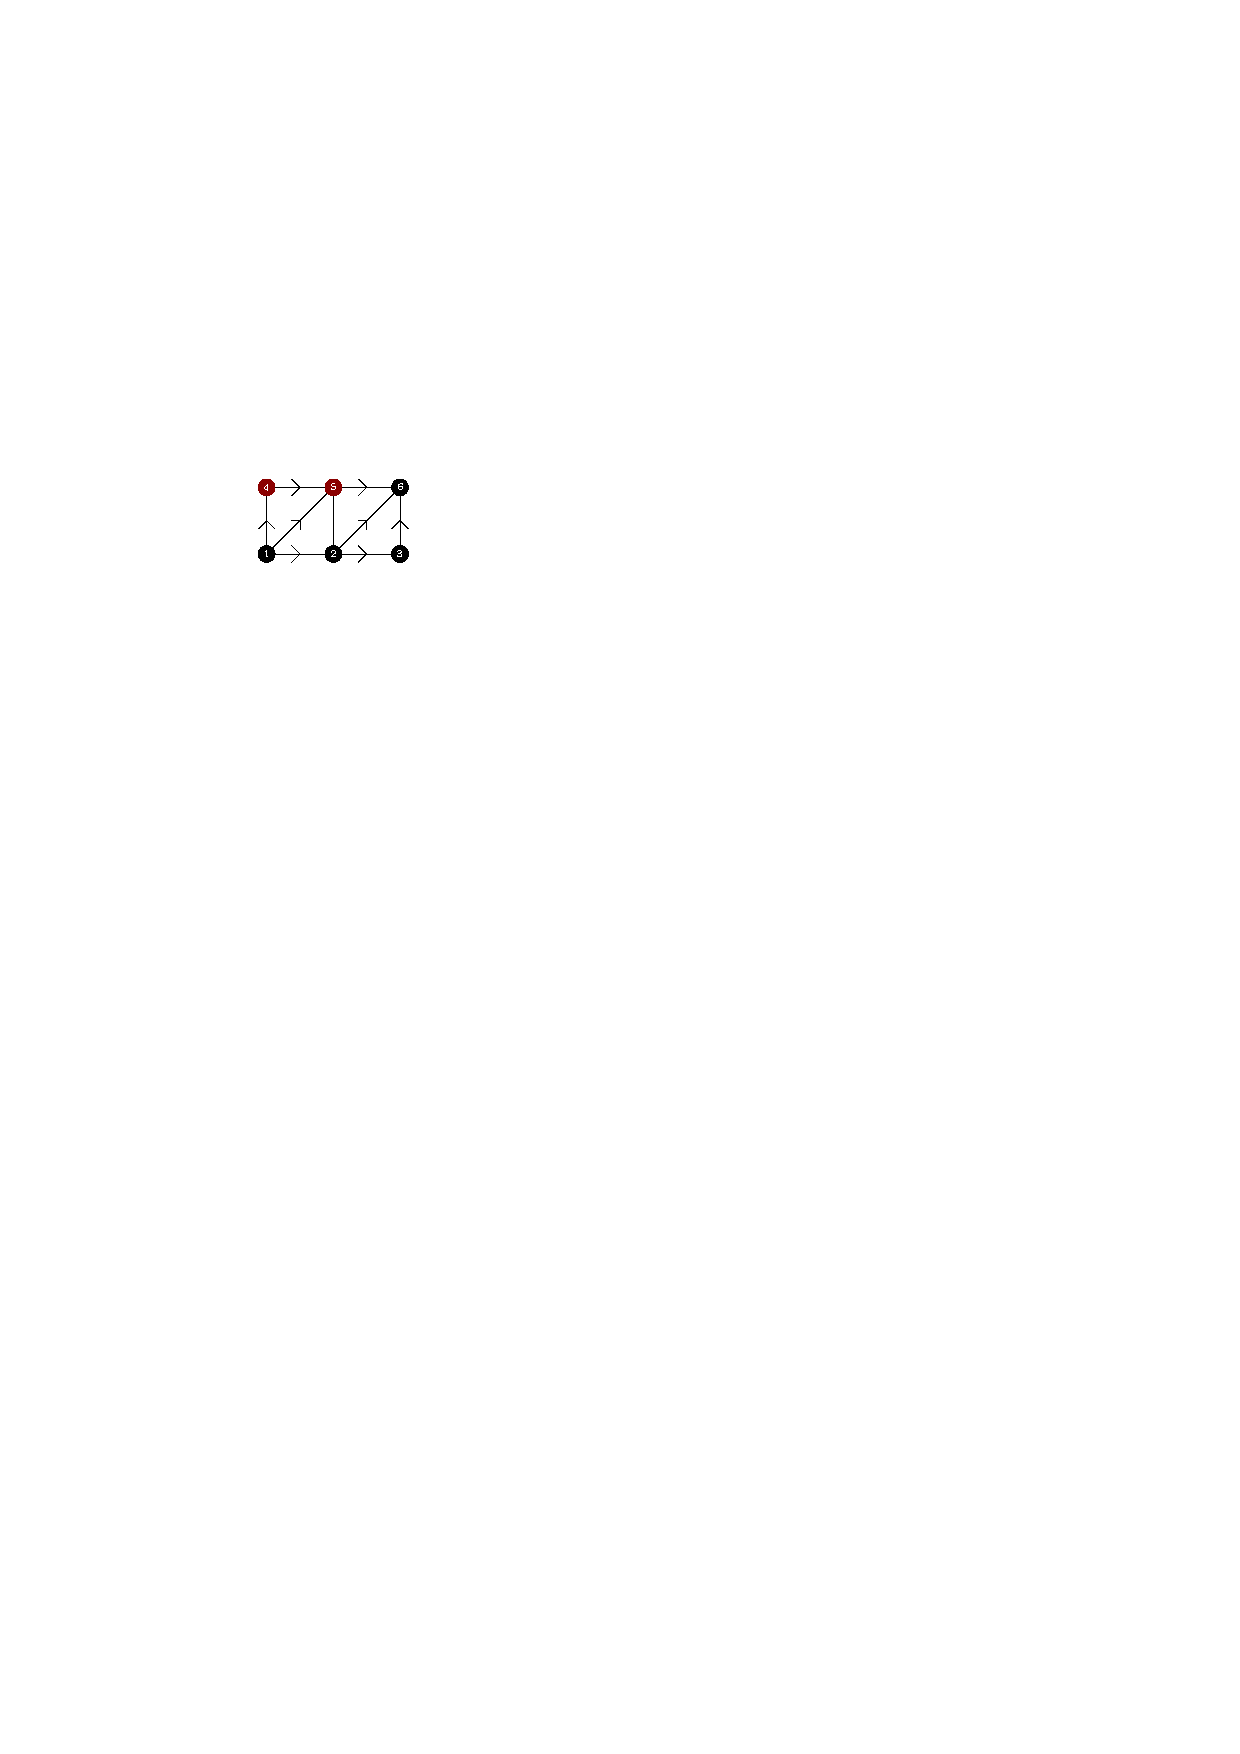
\includegraphics[width=0.8\linewidth]{images/F2.pdf}
        \end{figure}
    \end{column}
    \end{columns}
    \pause
    As \(2(n-2)(2n-3)<(2n-3)^2\) there exists a row with at least \(n-1\) red or a column with \(n-1\) blue points.\\
    \medskip
    Assume there is a row  with red points at \(j_1 < \cdots < j_{n-1}\)
Consider the columns
\vspace{-0.5cm}
\[
j_1,\dots,j_{n-1}, j_{n-1}+1,
\]
\vspace{-0.5cm}\\
Together with rows \(i,i+1\), this forms a \(2\times n\) subarray.\\

By monotonicity these rows and columns yield a type \(\mathcal{N}\) lex--monotone subarray.
\end{frame}

\begin{frame}{}
    \begin{lemma}{Lemma}
        For \(n \geq 3\), there exists an increasing array \(g\) of size \((n-1)(n-2)\times (n-1)^2\) such that
        \begin{itemize}
            \item \(g\) does not contain an \((n-1) \times 2\) subarray of type \(\mathcal{N}\)
            \item \(g\) does not contain an \(n \times 2\) subarray of type \(\mathcal{Z}\)
        \end{itemize}
    \end{lemma}
    \begin{columns}
    \begin{column}{0.5\linewidth}
        \only<1>{
        We take an array \(g\) partitioned into \(C_i\) such that
        \begin{itemize}
            \item \(C_1 < \dots < C_{n-2}\)
            \item Each \(C_i\) is of type \(\mathcal{Z}\).
        \end{itemize}
        }
        \only<2->{
        We can notice that:
        \begin{itemize}
            \item \((n-1) \times 2\) subarray of type \(\mathcal{N}\) would need to intersect in \(2\times 2\) with some \(C_i\), but \(C_i\) is type \(\mathcal{Z}\)
            \only<3>{
            \item \(n \times 2\) subarray of type \(\mathcal{Z}\) would need to intersect two seperate \(C_i\) thus it would contain \(2\times 2\) of type \(\mathcal{N}\)
            }
        \end{itemize}
        }
    \end{column}
    \begin{column}{0.5\linewidth}
        \vspace{-1cm}
        \begin{figure}
            \centering
            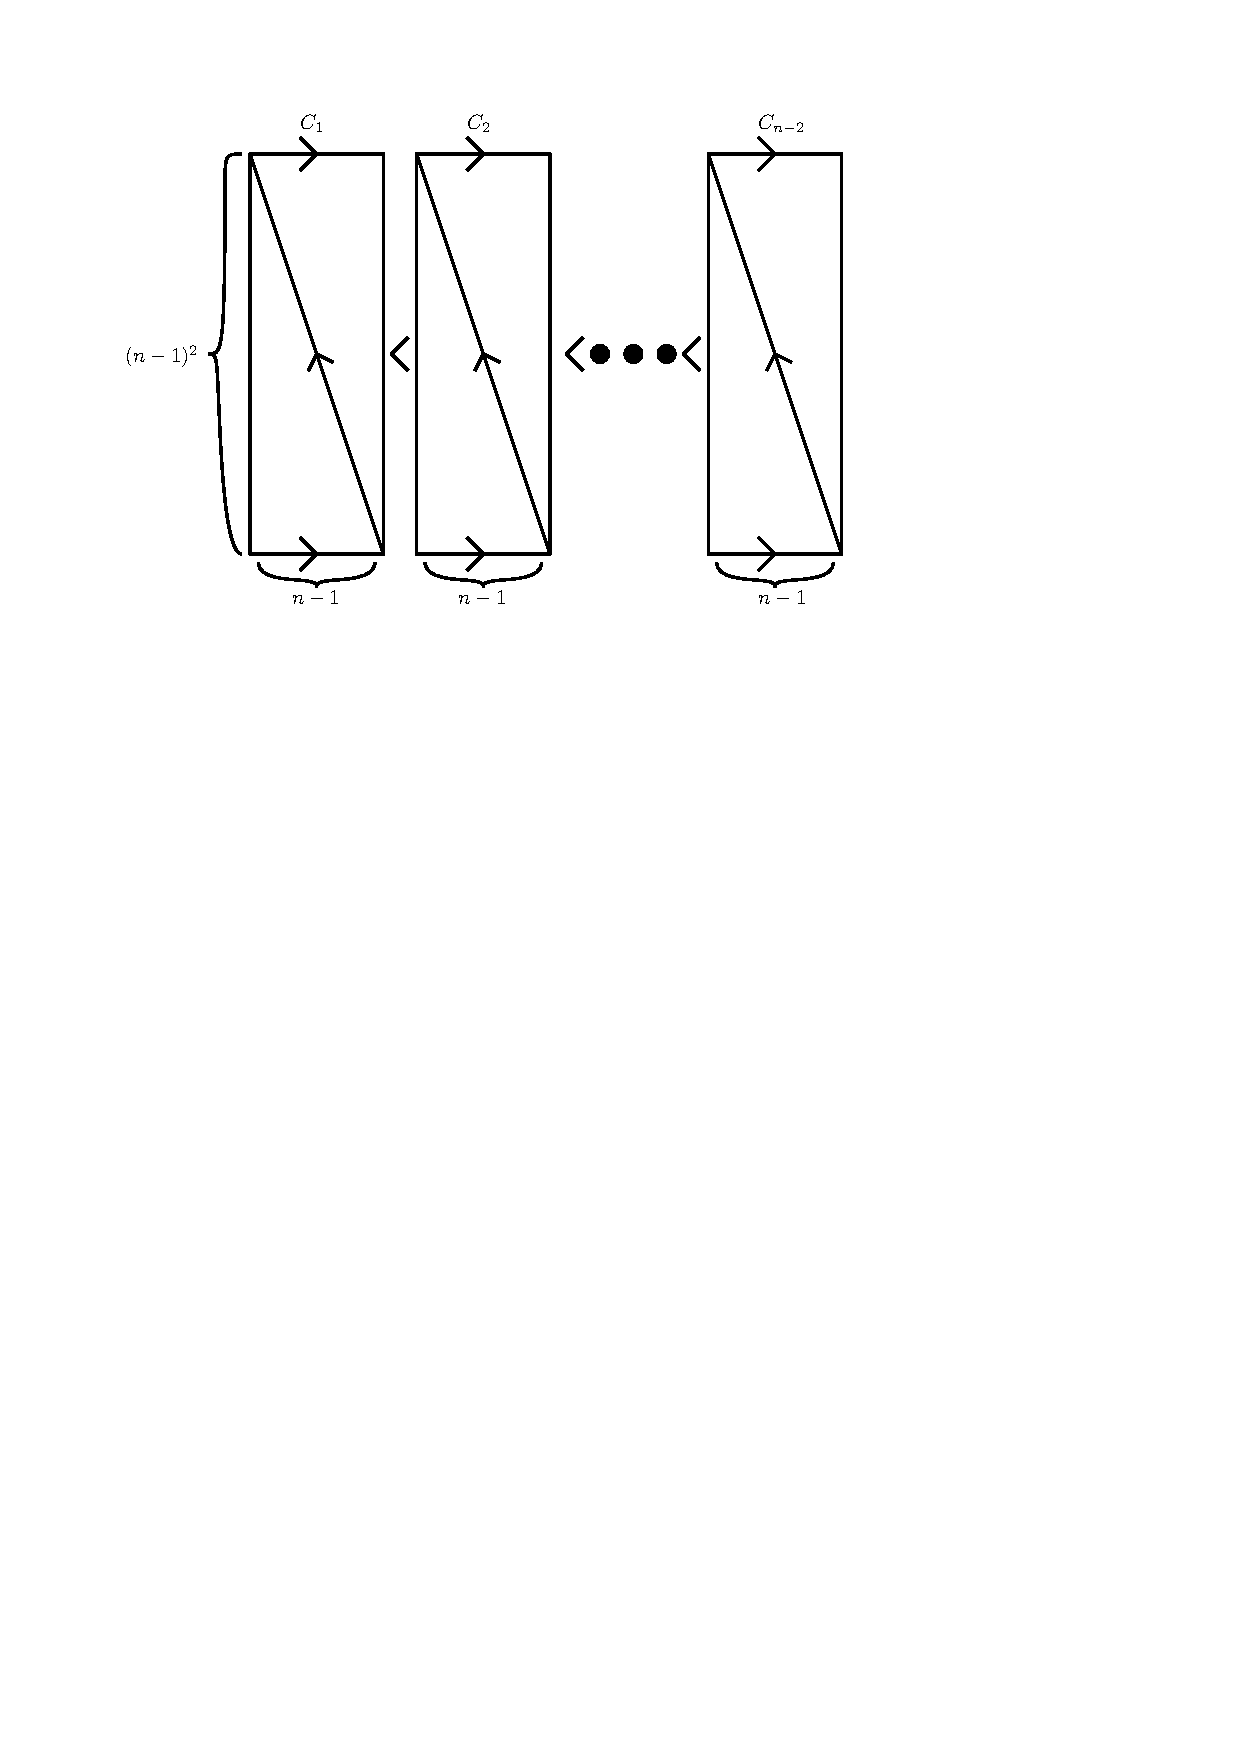
\includegraphics[width=\linewidth]{images/F_2_lower.pdf}
        \end{figure}
    \end{column}
    \end{columns}
\end{frame}


\begin{frame}{}
      \begin{lemma}{Lemma}
        For \(n \geq 3\), there exists an increasing array \(g\) of size \((n-1)(n-2)\times (n-1)^2\) such that
        \begin{itemize}
            \item \(g\) does not contain an \((n-1) \times 2\) subarray of type \(\mathcal{N}\)
            \item \(g\) does not contain an \(n \times 2\) subarray of type \(\mathcal{Z}\)
        \end{itemize}
    \end{lemma}

    \begin{lemma}{Lemma}
        For \(n \geq 3\), there exists an increasing array \(h\) of size \((n-1)^2 \times (n-1)(n-2)\) such that
        \begin{itemize}
            \item \(h\) does not contain an \(2 \times (n-1) \) subarray of type \(\mathcal{N}\)
            \item \(h\) does not contain an \(2  \times N\) subarray of type \(\mathcal{Z}\)
        \end{itemize}
    \end{lemma}
\end{frame}
\begin{frame}{}
    \begin{columns}
    \begin{column}{0.5\linewidth}
        Similarly we can show that if \(N=2n^2-5n+3\) we can construct an \(N\times N\) grid which does not contain an \(n \times n\) subgrid of types \(\mathcal{N}\) nor \(\mathcal{Z}\)\\
        \medskip 
        \begin{proof}{Proof sketch}
                We take 2 copies of \(g\) and two of \(h\) to form an \(n\times n\) grid (we fill the remains with an increasing array)
        \end{proof}
        \medskip
        \only<2>{
        \begin{theorem}{Lower bound}
            \(F_2(n)\geq 2n^2-5n+3\)
        \end{theorem}
        }
    \end{column}
    \begin{column}{0.5\linewidth}
        \begin{figure}
            \centering
            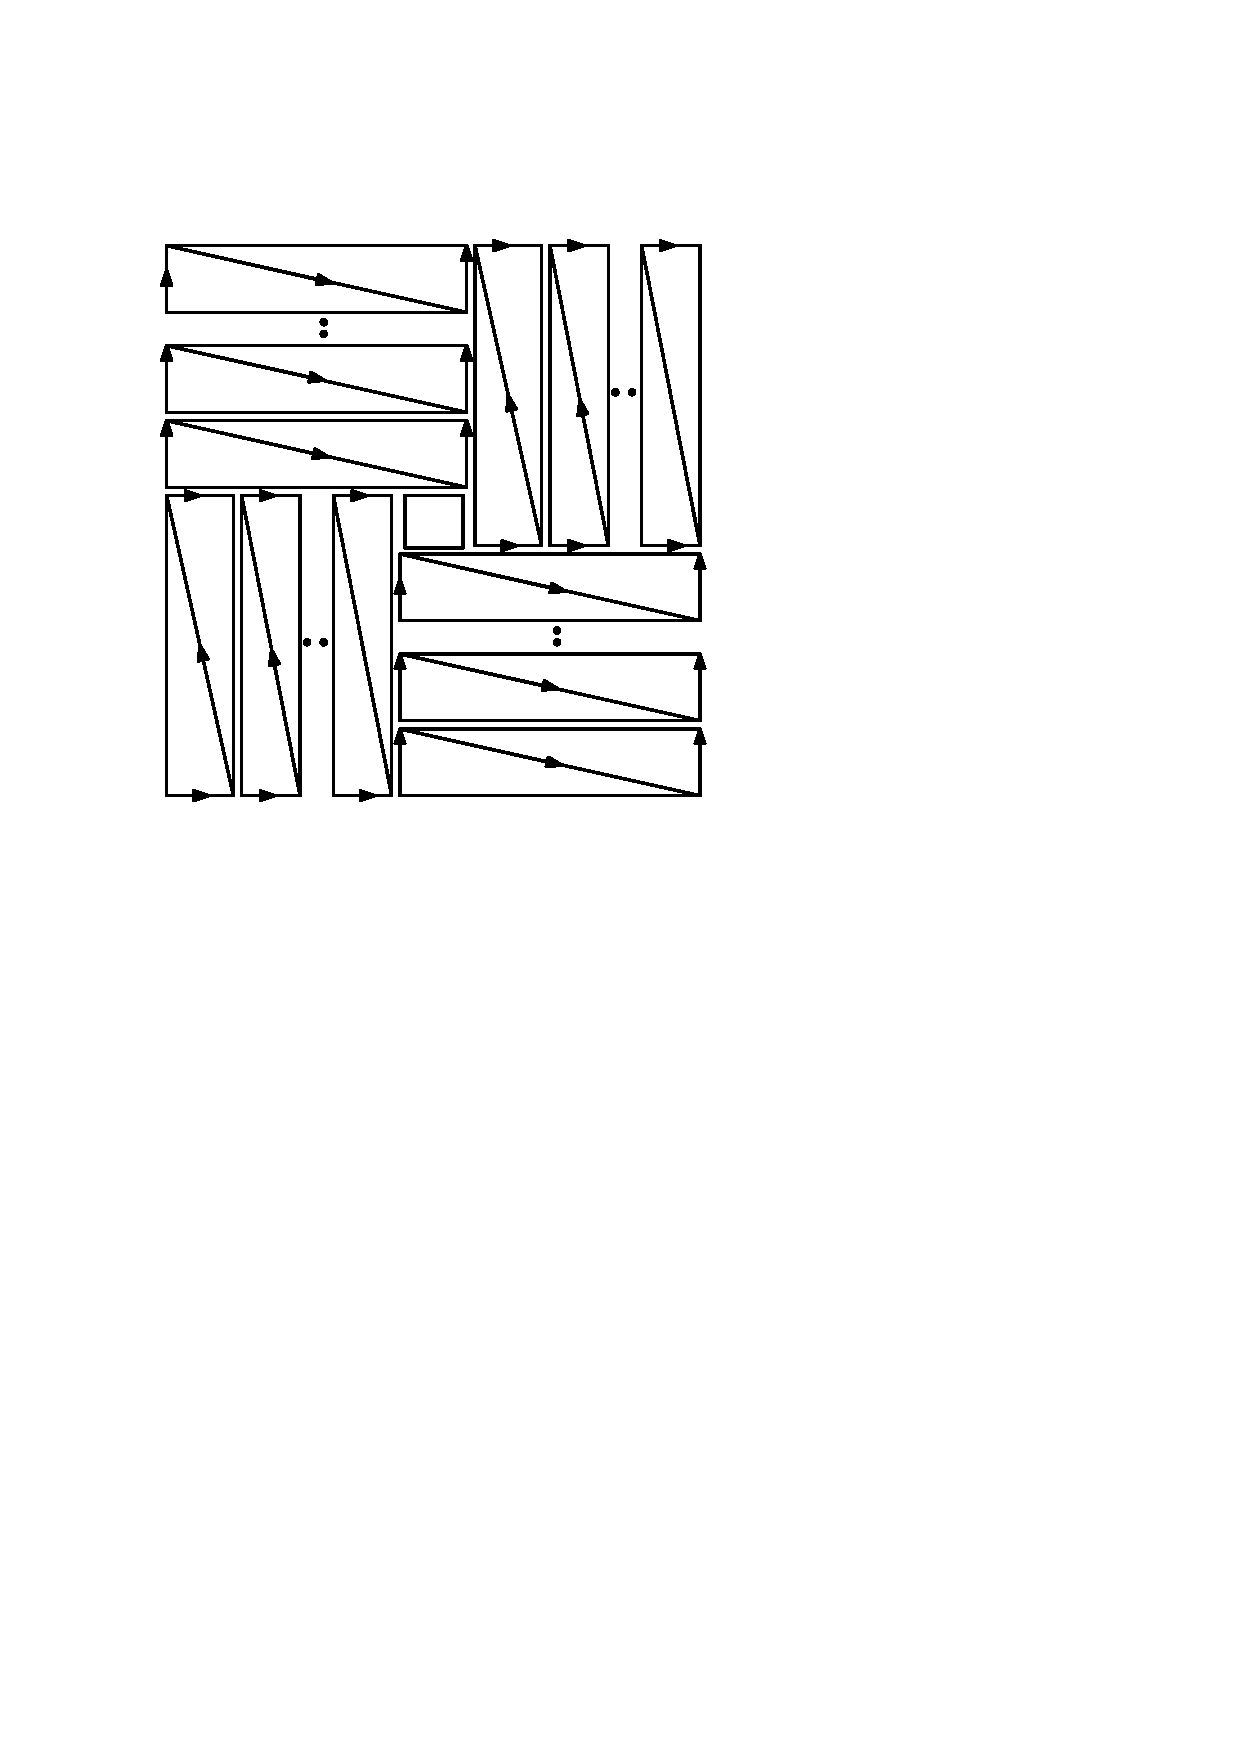
\includegraphics[width=0.8\linewidth]{images/weird.pdf}
        \end{figure}
    \end{column}
    \end{columns}
\end{frame}
\begin{frame}{}
    Through similar idea we can show the bound
    \begin{theorem}{High dimensional bound on \(F\)}
        \[F_d(n)\leq 2^{\left(\frac{1}{2}(d-1)!+o(1)\right)n^{d-2}}\leq 2^{O_d(n^{d-2})}\]
    \end{theorem}
    If we combine it with 
    \begin{theorem}{Bound on \(M_d\)}
        \[M_d(n)\leq 2^{2^{2^{O(n^{d-1})}}}\]
    \end{theorem}
    \pause 
    \begin{theorem}{Bound on $L_d(n)$}
        \[L_d(n) \leq M_d(F_d(n)) \leq 
        \underbrace{2^{2^{2^{O_d\left(2^{O_d(n^{d-2})}\right)}}}}_{\text{quadruple exp}}
        = \underbrace{2^{2^{2^{2^{O_d(n^{d-2})}}}}}_{\text{towr}_5(O_d(n^{d-2}))}\]
    \end{theorem}
\end{frame}


\section{Conclusions}
% \begin{frame}{Open questions}
%     \begin{itemize}
%         \item \(\text{exponent} \leq M_2(n) \leq \text{ double exponent}\)
%         \\Question: Do we need the double exponent at all?
%         \item \(M_d(n)\overset{?}{\leq} \text{ double exponent}\)
%         \item \(\text{polynomial }\leq F_d(n)  \leq \text{double exponent}\)
%         \\Question:  Do we need the double exponent at all?

%     \end{itemize}
    
% \end{frame}
\begin{frame}{Framing it as Ramsey}
    We can frame problems from this paper in the framework of Ramsey numbers.\\
    Take an array \(f:[N]^2\to \mathbb{R}\)  and a hypergraph \(K^3_{N,N}\) of the form \(A \cup B\) with a red, blue colouring edge \(\chi\):
    \begin{columns}
    \begin{column}{0.6\linewidth}
        
    \[\chi(i,j,j')=\begin{cases}
        \text{red if }\space\space  f(i,j)< f(i,j')\\
        \text{blue if }f(i,j)\geq f(i,j') 
    \end{cases}\]
    \end{column}
    \begin{column}{0.3\linewidth}
        \begin{figure}
            \centering
            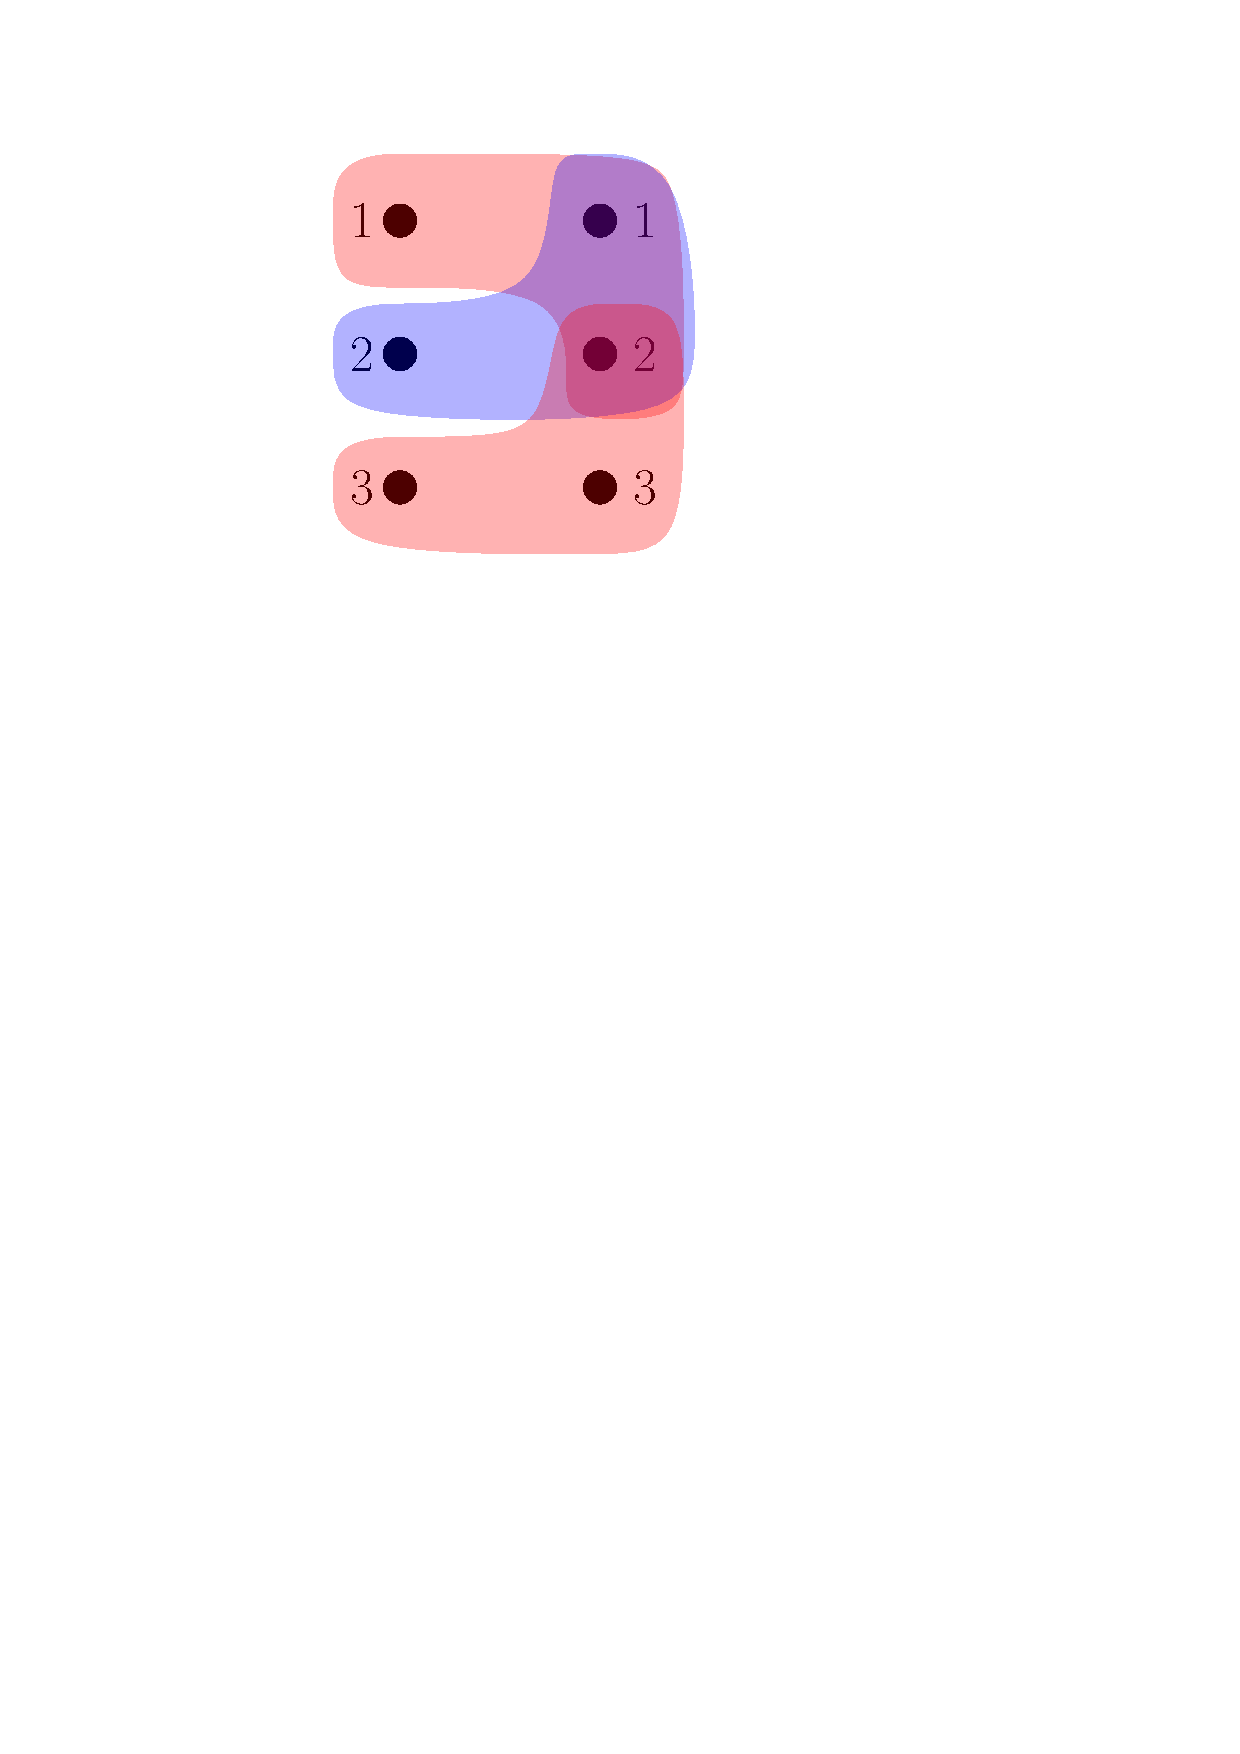
\includegraphics[width=0.5\linewidth]{images/like_ramsey.pdf}
        \end{figure}
    \end{column}
    \end{columns}

    \pause
    Suppose there are two size subsets \(\tilde{a} \subseteq A\) and \(\tilde{b} \subseteq B\) s.t.
    \begin{itemize}
        \item \(\set{a_i, b_j, b_{j+1}}\) is monochromatic under \(\chi\)
        \item \(\set{a_i, a_{i+1}, b_{j}}\) is monochromatic under \(\chi\)
    \end{itemize}
    then \(f\) is a monotone array when restricted to \(\tilde{a}\times \tilde{b}\)
\end{frame}


\begin{frame}{Summary of Bounds}
  \renewcommand{\arraystretch}{1.4}
  \begin{center}
    \begin{tabular}{lccc}
      \toprule
      & \( M_d(n) \) (monotone) & \( F_d(n) \) (mono→lex) & \( L_d(n) \) (lex) \\
      \midrule
      \( d=1 \) & \( (n-1)^2+1 \) & \( 1 \) & \( (n-1)^2+1 \) \\
      \( d=2 \) & \( 2^{2^{(2+o(1))n}} \) & \( 2n^2-5n+4 \) & \( 2^{2^{(4+o(1))n^2}} \) \\
      \( d=3 \) & \( 2^{2^{(2+o(1))n^2}} \) & \( 2^{O(n)} \) & \( 2^{2^{2^{O(n)}}} \) \\
      \( d \geq 4 \) & \( 2^{2^{2^{O_d(n^{d-1})}}} \) & \( 2^{O_d(n^{d-2})} \) & \( \text{towr}_5(O_d(n^{d-2})) \) \\
      \midrule
      lower bd & \multicolumn{3}{c}{\( M_d(n) \geq n^{(1-1/d)n^{d-1}} \)} \\
      \bottomrule
    \end{tabular}
  \end{center}
\end{frame}

\begin{frame}{Open Problems}
  \begin{ffact}{Main open problem}
    What is the order of magnitude of \( M_2(n) \)?
    Is it closer to \emph{exponential} or \emph{double exponential} in \( n \)?
  \end{ffact}
\pause
  \begin{ffact}{Question 4.2}
    For \( d \geq 4 \), is \( M_d(n) \) bounded by a \emph{double exponential}
    in \( n^{d-1} \)?
  \end{ffact}
\pause
  \begin{ffact}{Question 4.3}
    What is the smallest \( N \) such that, given \( N \) increasing \( N \times N \)
    arrays, one can find an \( n \times n \) lex-monotone pattern appearing in the
    same positions in at least \( n \) of the arrays?
    Is \( N \) polynomial or exponential in \( n \)?
  \end{ffact}
\end{frame}
% \begin{frame}{Other generalisations}
%     \begin{theorem}{Theorem (Suk, 2017)}
%         Any \(2^{n+o(n)}\) points in \(\mathbb{R}^2\) contain a convex subset of size \(n\).
%     \end{theorem}
%     \medskip
%     \pause
% \begin{theorem}{Theorem (Xu, 2024)}
% % Any sequence of \(n\) pairwise distinct real numbers contains a \(k\)-
% % modal subsequence of length at least
% % \(\sqrt{(2k + 1)(n − \frac{1}{4} )} - \frac{k}{2}\)
% % \end{theorem}
% % A k-modal sequence is a sequence of real numbers that can be partitioned into k + 1 (possibly
% % empty) monotone sections such that adjacent sections have opposite monotonicities. 
% \end{frame}



%---------------------------------------------------------
\begin{frame}{Sources}
\label{references}
    \begin{itemize}
        \item Matija Bucić, Benny Sudakov,  Tuan Tran --  \href{https://arxiv.org/pdf/2301.02020}{\textit{Erdős Szekeres theorem for multidimensional arrays}}, 2022. \\
    \end{itemize}
  \centering
  \Large \textbf{Thank you!}
\end{frame}

%---------------------------------------------------------


\end{document}